\documentclass[letterpaper,12pt]{article}
\usepackage{array}
\usepackage{threeparttable}
\usepackage{geometry}
\geometry{letterpaper,tmargin=1in,bmargin=1in,lmargin=1.25in,rmargin=1.25in}
\usepackage{fancyhdr,lastpage}
\pagestyle{fancy}
\lhead{}
\chead{}
\rhead{}
\lfoot{}
\cfoot{}
\rfoot{\footnotesize\textsl{Page \thepage\ of \pageref{LastPage}}}
\renewcommand\headrulewidth{0pt}
\renewcommand\footrulewidth{0pt}
\usepackage[format=hang,font=normalsize,labelfont=bf]{caption}
\usepackage{listings}
\usepackage{booktabs}
\lstset{frame=single,
  language=Python,
  showstringspaces=false,
  columns=flexible,
  basicstyle={\small\ttfamily},
  numbers=none,
  breaklines=true,
  breakatwhitespace=true
  tabsize=3
}
\usepackage{amsmath}
\usepackage{amssymb}
\usepackage{amsthm}
\usepackage{harvard}
\usepackage{setspace}
\usepackage{float,color}
\usepackage[pdftex]{graphicx}
\usepackage{hyperref}
\usepackage{pgfplotstable}
\hypersetup{colorlinks,linkcolor=red,urlcolor=blue}
\theoremstyle{definition}
\newtheorem{theorem}{Theorem}
\newtheorem{acknowledgement}[theorem]{Acknowledgement}
\newtheorem{algorithm}[theorem]{Algorithm}
\newtheorem{axiom}[theorem]{Axiom}
\newtheorem{case}[theorem]{Case}
\newtheorem{claim}[theorem]{Claim}
\newtheorem{conclusion}[theorem]{Conclusion}
\newtheorem{condition}[theorem]{Condition}
\newtheorem{conjecture}[theorem]{Conjecture}
\newtheorem{corollary}[theorem]{Corollary}
\newtheorem{criterion}[theorem]{Criterion}
\newtheorem{definition}[theorem]{Definition}
\newtheorem{derivation}{Derivation} % Number derivations on their own
\newtheorem{example}[theorem]{Example}
\newtheorem{exercise}[theorem]{Exercise}
\newtheorem{lemma}[theorem]{Lemma}
\newtheorem{notation}[theorem]{Notation}
\newtheorem{problem}[theorem]{Problem}
\newtheorem{proposition}{Proposition} % Number propositions on their own
\newtheorem{remark}[theorem]{Remark}
\newtheorem{solution}[theorem]{Solution}
\newtheorem{summary}[theorem]{Summary}
%\numberwithin{equation}{section}
\bibliographystyle{aer}
%\newcommand\ve{\varepsilon}
%\newcommand\boldline{\arrayrulewidth{1pt}\hline}


\begin{document}

\begin{flushleft}
  \textbf{\large{Problem Set \#[3]}} \\
  MACS 40000, Dr. Evans \\
  Fiona Fan
\end{flushleft}

\vspace{5mm}

\noindent\textbf{Problem 1}
\\ \textbf{Part (a).} The first period consumption, $c_1$ is negative, most possibly resulted from a excessively big $b_1$.
\\ \textbf{Part (b).} No constraint is violated.
\\ \textbf{Part (c).} No constraint is violated.\\




\noindent\textbf{Problem 2} \\
\textbf{Part (a).} Please see Column B and D of $problem2.csv$ for $\{{b_t}_{t=1}^{S}\}$ and $\{{c_t}_{t=1}^{S}\}$. $\bar{K}$ and $\bar{L}$ are 494.14 and 58.4, and $\bar{w}$ and $\bar{r}$ are 1.37 and 0.037 respectively. The computations took 0.046s and 0.083s.

\textbf{Part (b).} Please see Figure \ref{Fig1}. 

\textbf{Part (c).} 
\par See the Column C and E of $problem2.csv$ and \ref{Fig2} for $\{{b_t}_{t=1}^{S}\}$ and $\{{c_t}_{t=1}^{S}\}$. $\bar{K}$ and $\bar{L}$ change 565.88 and 48 respectively, and $\bar{w}$ and $\bar{r}$ change to 1.54 and 0.02. For both, once the agents retire, they cut their savings to keep their consumption at a near constant level. For agents that retire earlier, they cut happens earlier. The maximum amount of saving for when $n=2/3$ is 15.29, and when $n=1/2$, then maximum is 16.45. On average before the cut the agents in $n=1/2$ case save more to reach that higher maximum. And on average teh agents in the $n=2/3$ case consume and save more because they have worked more and have more money. 

\textbf{Part (c).} 
\par Since $c_{s,t}=(1+r_t)b_{s,t}+w_t n_s-b_{s+1,t+1}$, there should be a lower bound for $b_{s,t}$ and an upper bound for $b_{s+1,t+1}$ to keep $c_{s,t}$ positive.

\noindent\textbf{Problem 3}\\
\textbf{Part (a).} Please see Figure \ref{Fig3}, Figure \ref{Fig4} and Figure \ref{Fig5} for $\{{K_t}_{t=1}^{T+5}\}$, $\{{w_t}_{t=1}^{T+5}\}$ and $\{{r_t}_{t=1}^{T+5}\}$ respectively.

\noindent\textbf{Part (b).} Please see Figure \ref{Fig6} for $\{{b_{15,t}}_{t=1}^{T+5}\}$. $b_{15,t}$ rises above $\bar{b_15}$ 220 times. The first time appears at period 2. 

\noindent\textbf{Part (c).} In period 219, the economy first gets to within 0.00001 of the steady state. After period 320, which is the last period, the economy is never again father than 0.00001 away from the steady state. That means within each agents' lifetime, K does not get within the threshold approximating $K_ss$. 



\begin{figure}[htb]\centering
	\captionsetup{width=4.0in}
	\caption{\textbf{Steady-State Distribution of Consumption and Savings by Age when $n=2/3$}}
	\label{Fig1}
	\fbox{\resizebox{4.0in}{3.0in}{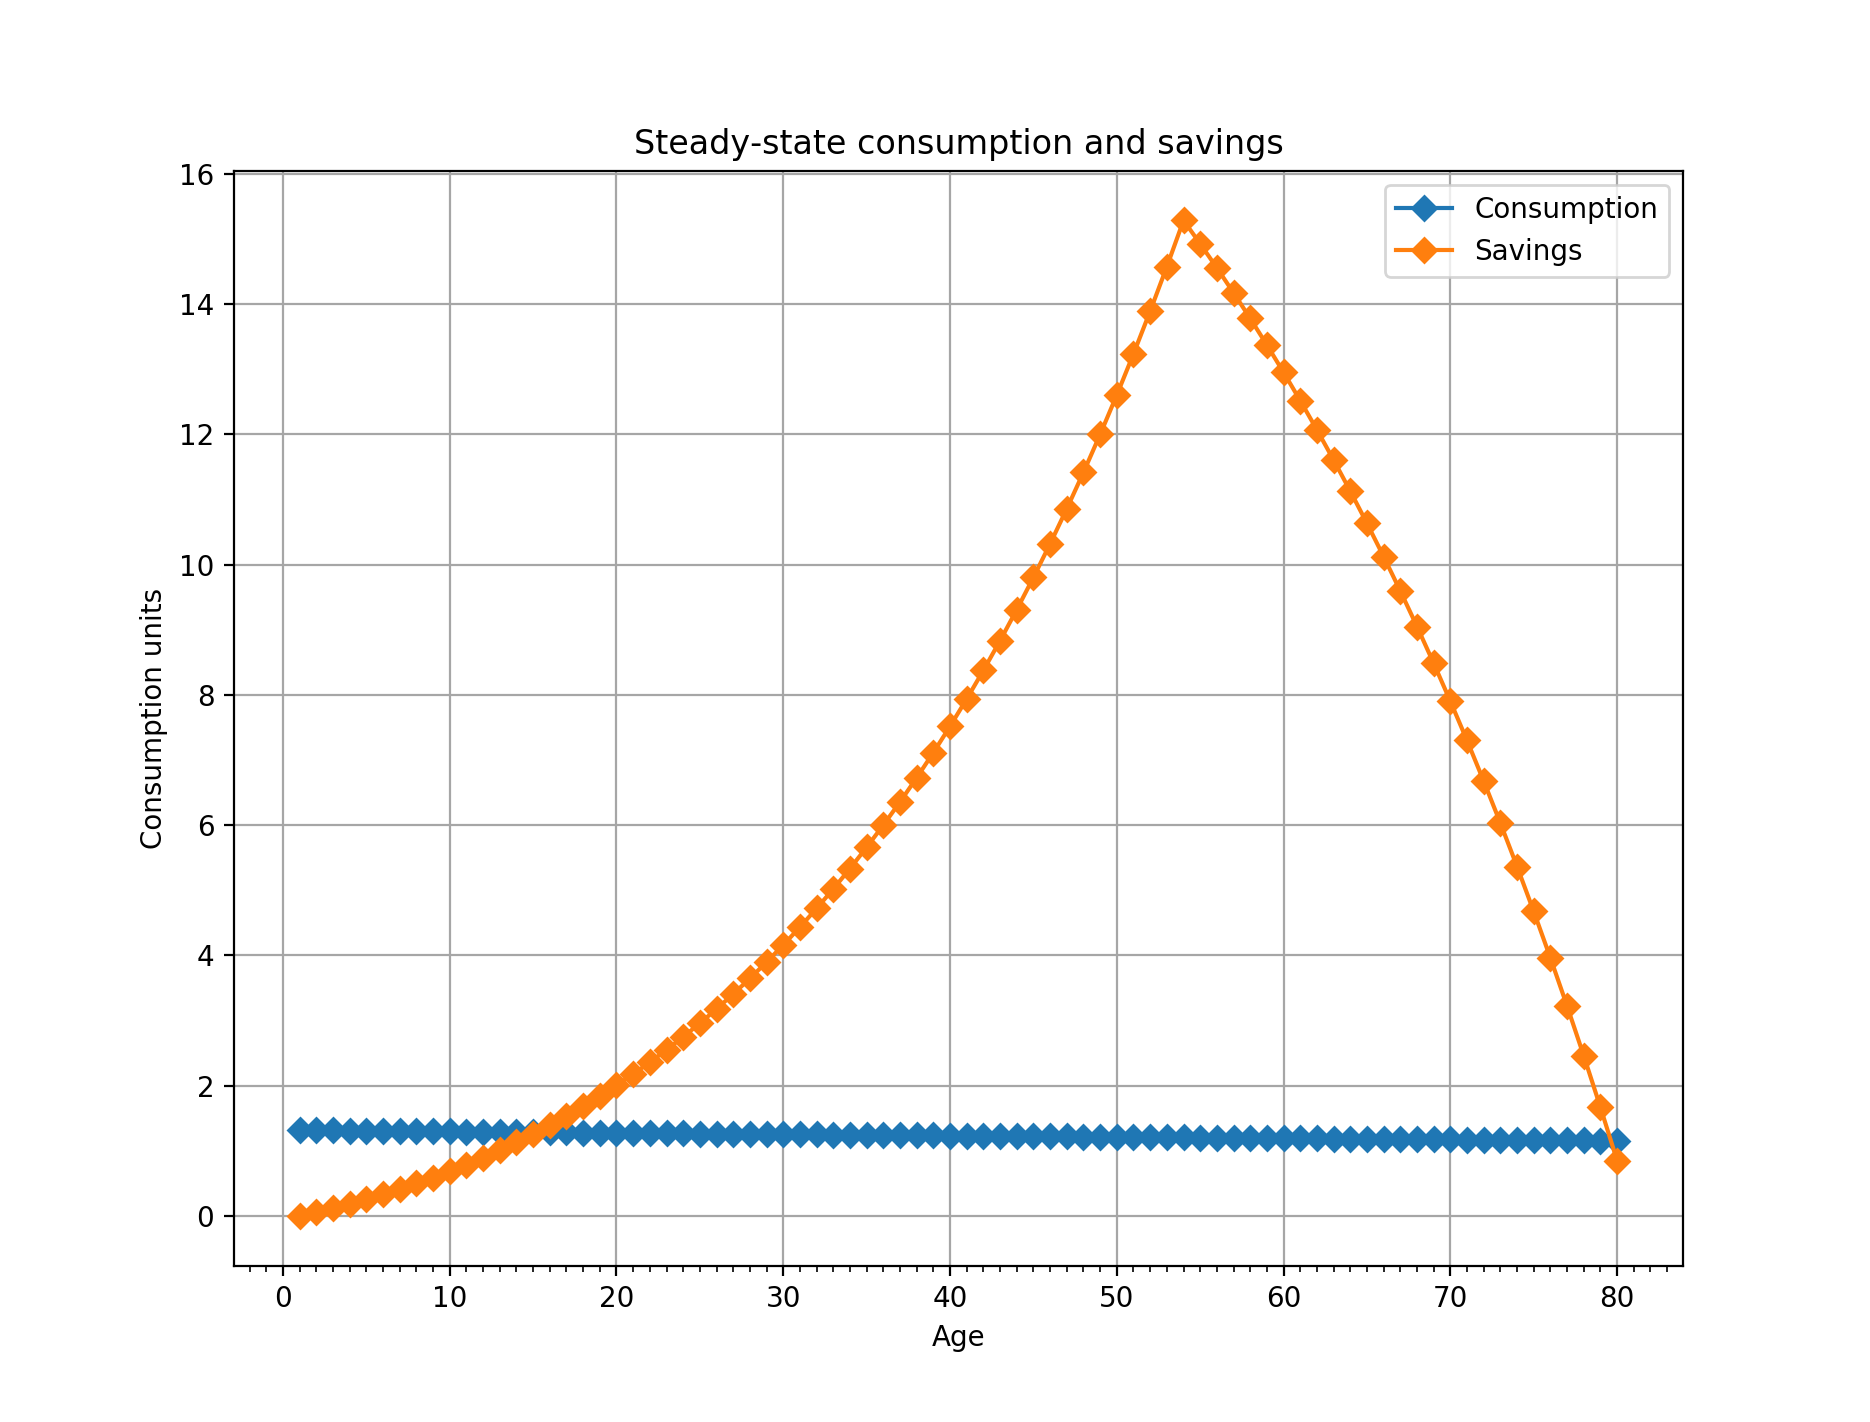
\includegraphics{images/n1.png}}}
\end{figure}

\begin{figure}[htb]\centering
	\captionsetup{width=4.0in}
	\caption{\textbf{Steady-State Distribution of Consumption and Savings by Age when $n=1/2$}}
	\label{Fig2}
	\fbox{\resizebox{4.0in}{3.0in}{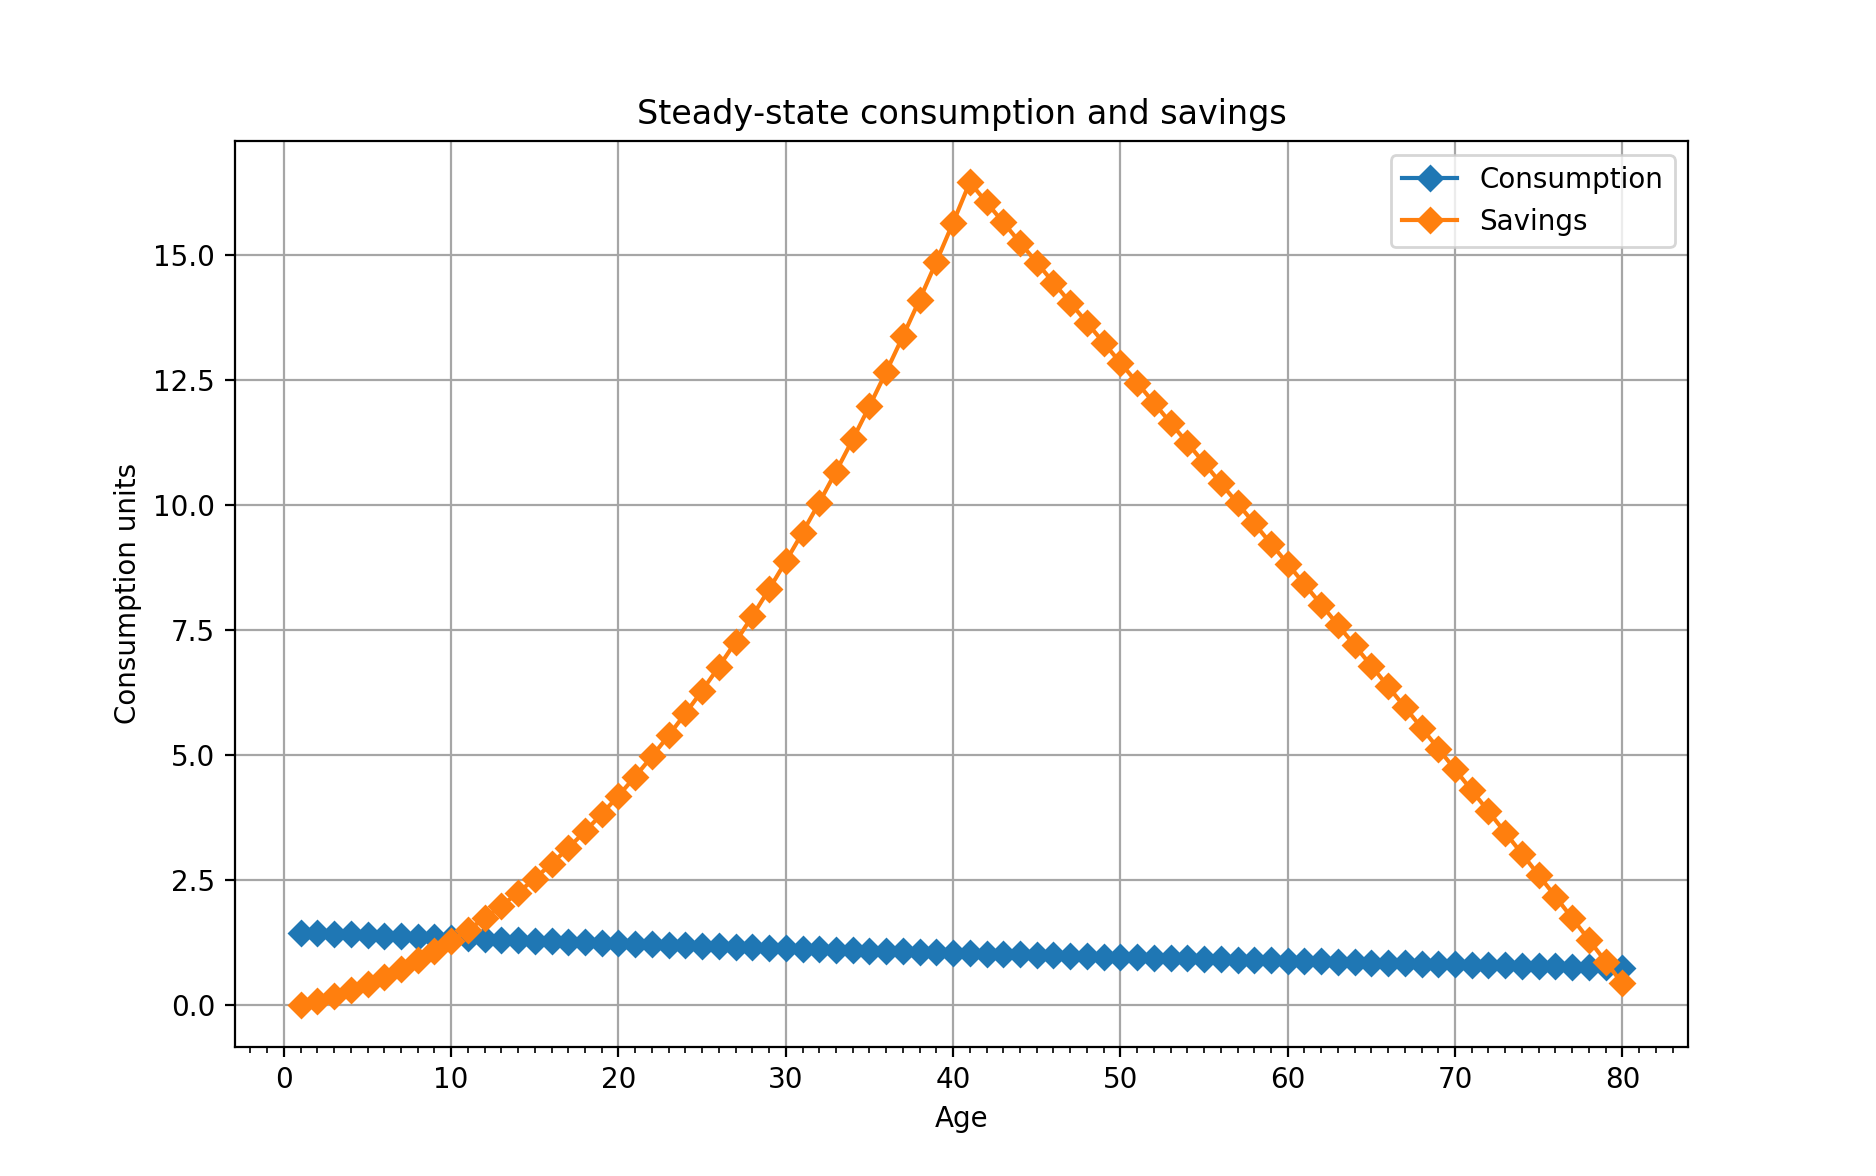
\includegraphics{images/n2.png}}}
\end{figure}

\begin{figure}[htb]\centering
	\captionsetup{width=4.0in}
	\caption{\textbf{$\{{K_t}_{t=1}^{T+5}\}$}} \label{Fig3}
	\fbox{\resizebox{4.0in}{3.0in}{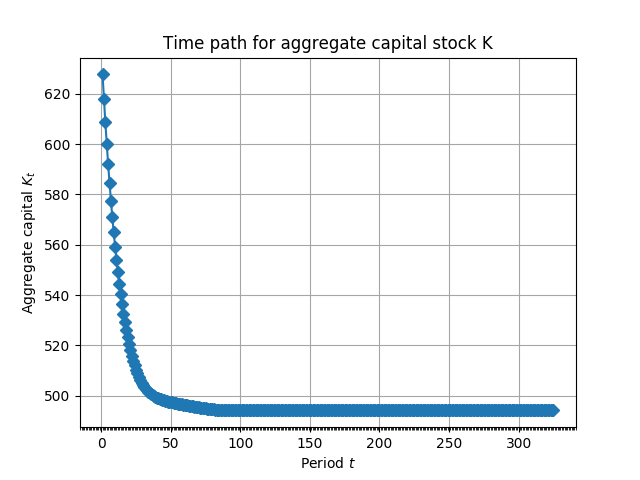
\includegraphics{images/Kpath.png}}}
\end{figure}

\begin{figure}[htb]\centering
	\captionsetup{width=4.0in}
	\caption{\textbf{$\{{w_t}_{t=1}^{T+5}\}$}}
	\label{Fig4}
	\fbox{\resizebox{4.0in}{3.0in}{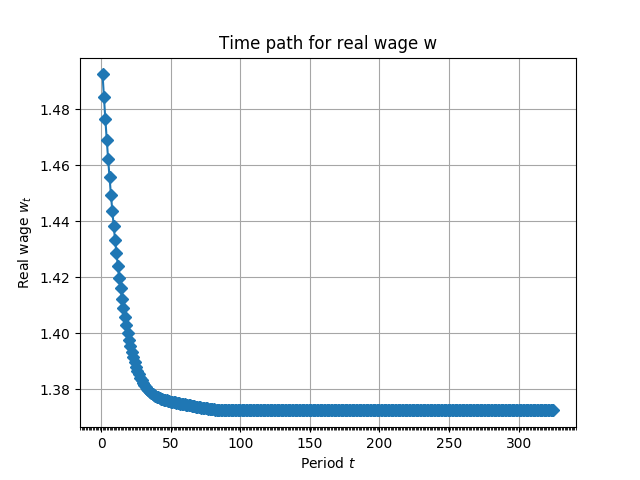
\includegraphics{images/wpath.png}}}
\end{figure}

\begin{figure}[htb]\centering
	\captionsetup{width=4.0in}
	\caption{\textbf{$\{{r_t}_{t=1}^{T+5}\}$}}
	\label{Fig5}
	\fbox{\resizebox{4.0in}{3.0in}{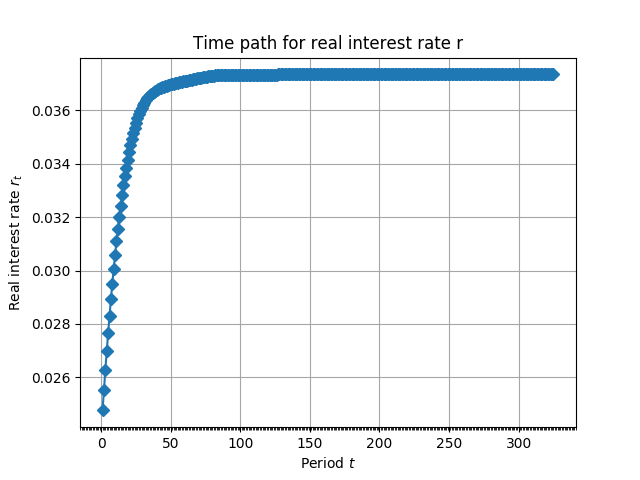
\includegraphics{images/rpath.png}}}
\end{figure}

\begin{figure}[htb]\centering
	\captionsetup{width=4.0in}
	\caption{\textbf{$\{{b_{15,t}}_{t=1}^{T+5}\}$}}
	\label{Fig6}
	\fbox{\resizebox{4.0in}{3.0in}{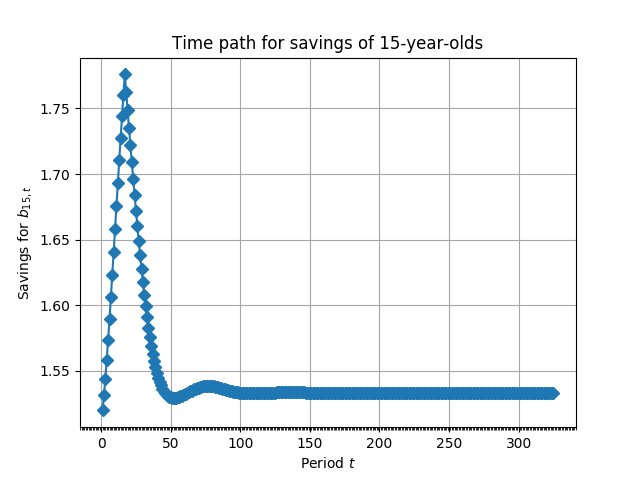
\includegraphics{images/b15path.png}}}
\end{figure}


\end{document}

